\documentclass[leqno,presentation]{beamer}
\DeclareGraphicsExtensions{.eps,.jpg,.png,.tif}
\usepackage{amssymb, amsmath, pdfpages, amsfonts, calc, times, type1cm, latexsym, xcolor, colortbl, hyperref, bookmark}
\usepackage{graphicx}
\usepackage{tabularx}
\usepackage{multirow}
\graphicspath{ {images/} }

\usepackage[latin1]{inputenc}
\usepackage[english]{babel}
\usetheme{Darmstadt}
\newcommand{\R}{\mathbb{R}}
\newcommand{\N}{\mathbb{N}}
\newcommand{\overbar}[1]{\mkern1.5mu\overline{\mkern-1.5mu#1\mkern-1.5mu}\mkern1.5mu}
\newcommand{\highlight}[1]{
  \addtolength{\fboxrule}{.2ex}
  \begin{block}{}
    \begin{quote}#1
    \end{quote}
  \end{block}
}

\newtheorem*{conjecture}{Conjecture}
\newtheorem*{proposition}{Proposition}

\title{Automatic Theorem Proving}
\author[names]{ Reed Oei, Eric Ma \\ Christian Schulz (Team Leader) \\ Philipp Hieronymi (Faculty mentor)}

\institute{
  \\[-3ex]
  University of Illinois at Urbana-Champaign
  \\[2ex]
  \includegraphics[width = 0.3\textwidth]{UIUC_logo.png}
  \hspace{.30cm}
  
\includegraphics[width = 0.07\textwidth]{igl-logo-small.png}
  \\[3ex]
  Illinois Geometry Lab  \\  Midterm Presentation\\ March 25, 2020\\[2ex] }

\date{}

\begin{document}
% Title slide
\frame{\titlepage}

\section{Theorem Proving}

\begin{frame}{Automatic Theorem Proving}
    \begin{itemize}
        \item An \emph{automated theorem prover} is a program that takes a statement and proves if it is true or false, or gives the condition for the statement to be true.
        
        \item Automated theorem provers have attractive qualities
            \begin{itemize}
                \item Computers are very reliable, and never get tired/bored
                \item Can easily explore of new hypotheses
            \end{itemize}
            
        \item With some restrictions, there are programs that can prove first order logic statements.
    \end{itemize}
\end{frame}

% Reed: Probably don't need to talk about Walnut anymore
% \begin{frame}{Walnut}
%     \begin{itemize}
%         \item Walnut is an automated theorem prover.
%         \begin{itemize}
%         \item Utilizes the closure property of automata.
%         \item Input: A first order logic statement of some predicates about finite words, and automata for these predicates.
%         \item Output: The condition for the statement to be true, or if the statement is always true or false.
%         \end{itemize}
%         \item 
%         \begin{tabular}{|c|c}
%         \cline{1-1}
%         Inputs:                                   & \multirow{3}{*}{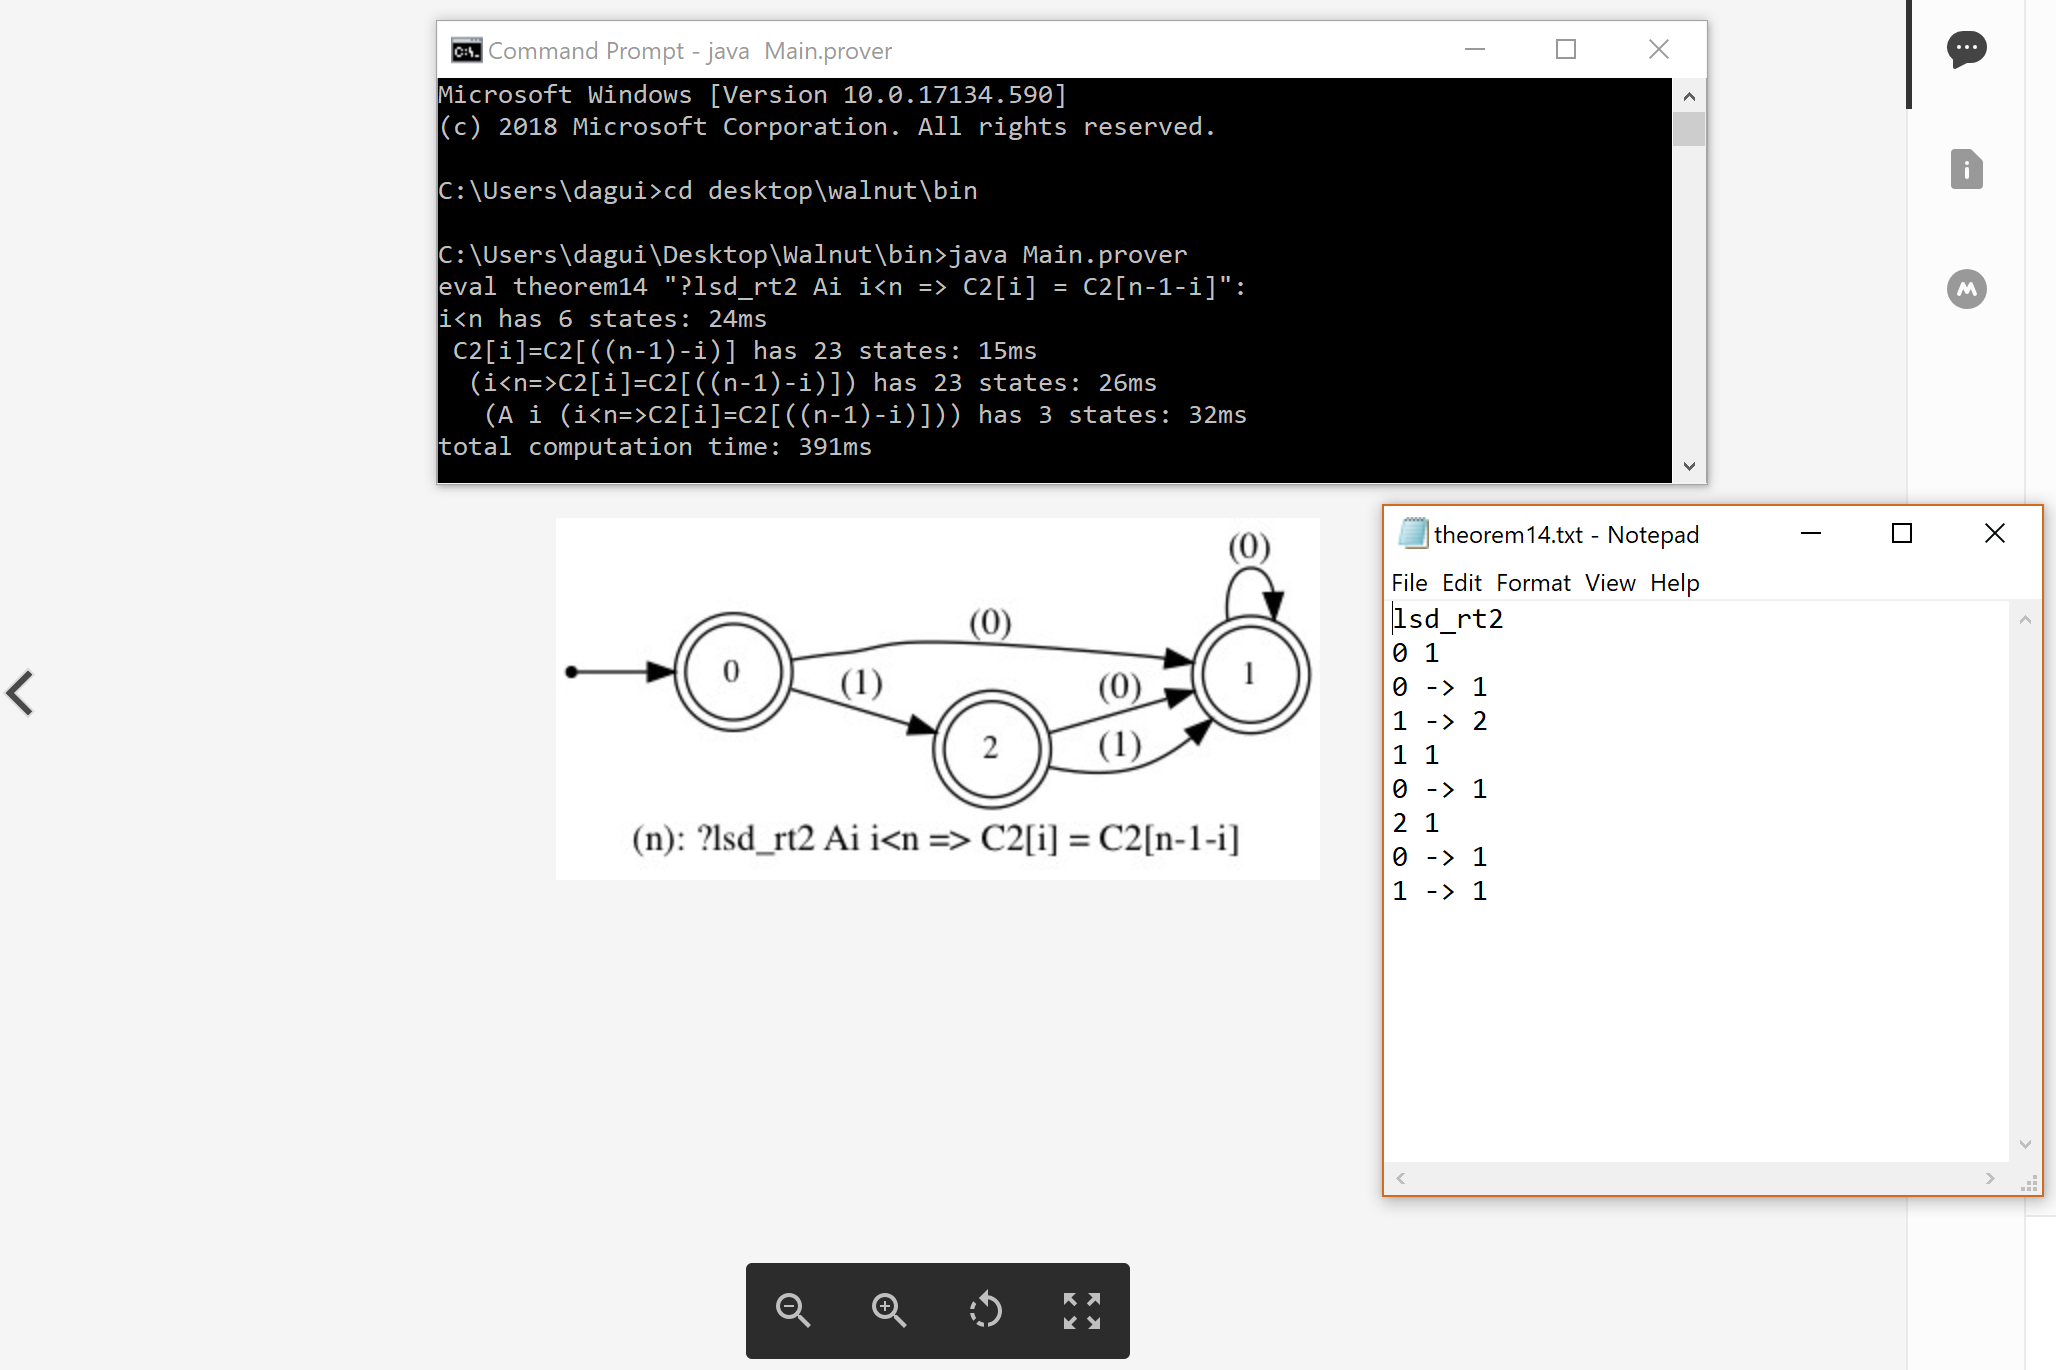
\includegraphics[width=0.5\linewidth]{Walnut.png}}\\\cline{1-1}
%         $p := \exists x (A(x,y) \land B(x))$,      &   \\
%         Automata for $A$ and $B$                  &   \\ \cline{1-1}
%         Output:                                   &   \\ \cline{1-1}
%         An automaton accepts        &   \\
%          $y$ that makes $p$ true                       &   \\ \cline{1-1}
%         \end{tabular}
        
%     \end{itemize}
% \end{frame}

\section{Sturmian Words}

\begin{frame}
    \frametitle{Sturmian Words}
    
    \begin{itemize}
        \item Imagine hitting a billiard ball at some angle $\theta$
        \item When the ball crosses a vertical line, write a 0; for horizontal lines, write a 1
        \item Each $\theta$ defines a \emph{characteristic Sturmian word}, $C_{\theta}$
        \item $C_{1/\phi} = 0100101001\ldots$
    \end{itemize}
    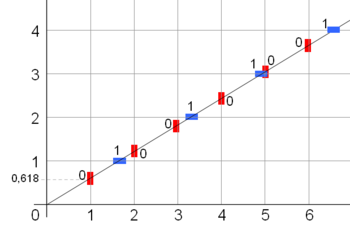
\includegraphics[height=0.4\textheight]{images/Fibonacci_word_cutting_sequence.png}
\end{frame}

\begin{frame}{Propositions about Sturmian Words}
    \begin{itemize}
        \item Questions about Sturmian words:
            \begin{itemize}
                \item Are they \emph{eventually periodic}?
                \item Are they \emph{balanced} (how similar are different sections of the word)?
                \item Do they contain \emph{palindromes}, and if so, what do the palindromes look like?
                \item Do they contain \emph{squares} (e.g., ``mama'', ``hotshots'')?
                \item Do they contain \emph{antisquares} (e.g., ``010101''), and if so, how many?
                \item And many more...
            \end{itemize}
            
        \item Conclusion: we need an automaton to calculate the digits of Sturmian words
    \end{itemize}
\end{frame}

% Reed: Probably don't need this
\begin{frame}
    \frametitle{Generating Sturmian Words}
    \begin{itemize}
        \item For each Sturmian word $C_{\alpha}$, there is an automaton that generates the $n$-th digit of the Sturmian word, $C_{\alpha}[n]$
            \begin{enumerate}
                \item Write $n$ in the Ostrowski-$\alpha$ numeration system
                \item Count the number of $0$s at the end of the string
                \item If odd, then $C_{\alpha}[n] = 1$; otherwise $C_{\alpha}[n] = 0$
            \end{enumerate}
            
        \item Because we can do arithmetic (e.g., addition) with numbers in their Ostrowski-$\alpha$ representation, automata can express many properties of Sturmian words
    
        \begin{figure}
            \centering
            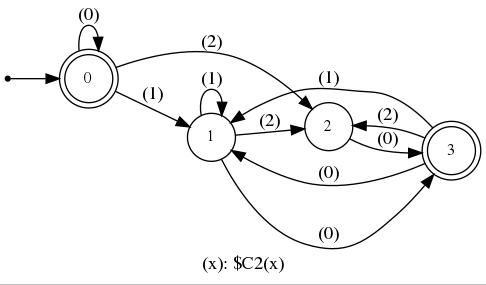
\includegraphics[height=0.5\textheight]{images/c2.jpg}
            \caption{An automaton that outputs $C_{\sqrt{2}}$}
            \label{fig:c2}
        \end{figure}
    \end{itemize}
\end{frame}

%         \item To calculate $C_{\sqrt{2}}[N]$:
%             \begin{itemize}
%                 \item Write $N$ in Ostrowski-$\sqrt{2}$
%                 \item Count the number trailing of $0$s, $\#_0(N)$
%                 \item $C_{\sqrt{2}}[N] = \#_0(N) \mod{2}$
%             \end{itemize}
    
%         \item $2 = 10_{\sqrt{2}} \mapsto 1$
%         \item $102 = 110011_{\sqrt{2}} \mapsto 0$
%     \end{itemize}
% \end{frame}

\section{Prior Work}

\begin{frame}{$k$-bounded Sturmian words}
    \begin{itemize}
        \item Last semester, we created automata that decide properties of so-called $k$-bounded Sturmian words: Sturmian words whose slopes' continued fraction has only coefficients bounded by some integer
        
        \item For example, $C_{\sqrt{3}}$ is a $2$-bounded Sturmian word:
        
        \[
            \sqrt{3} = 1 + \cfrac{1}{1 + \cfrac{1}{2 + \cfrac{1}{1 + \cfrac{1}{2 + \cdots}}}}
        \]

    \end{itemize}
\end{frame}

\begin{frame}{Prior Results}
    \begin{itemize}
        \item Last semester, we made several conjectures about various properties of Sturmian words, including:
        
            \begin{conjecture}\label{conj:antisq}
                Every Sturmian word has only finitely many antisquares.
            \end{conjecture}
                        
            \begin{conjecture}\label{conj:grouped}
                Every Sturmian word contains grouped factors.
            \end{conjecture}
        
        \item Using the automata we created and an automated theorem prover called Walnut, we proved statements for all $k$-bounded Sturmian words up to $k = 5$
        
        \item Limitation: Our current approach cannot prove the above for \textbf{all} Sturmian words
    \end{itemize}
\end{frame}

\section{Progress}

\begin{frame}
  \frametitle{Infinite Inputs}
  \begin{itemize}
      \item $\omega$-words are infinite length strings
      \begin{itemize}
          \item Example: $01001000100001...$
          \item Can represent real numbers
      \end{itemize}
      \item There are a couple types of automata that take $\omega$-words with different acceptance conditions
  \end{itemize}
\end{frame}

\begin{frame}{B\"uchi Automata}
    \begin{itemize}
          \item B\"uchi automata take $\omega$-words
          \item Accept sequences if they visit an accepting state infinitely often
          \item Corresponding statements are closed under first order logic operations (ex: and, or, $\forall$, $\exists$)
      \end{itemize}
       \begin{figure}
            \centering
            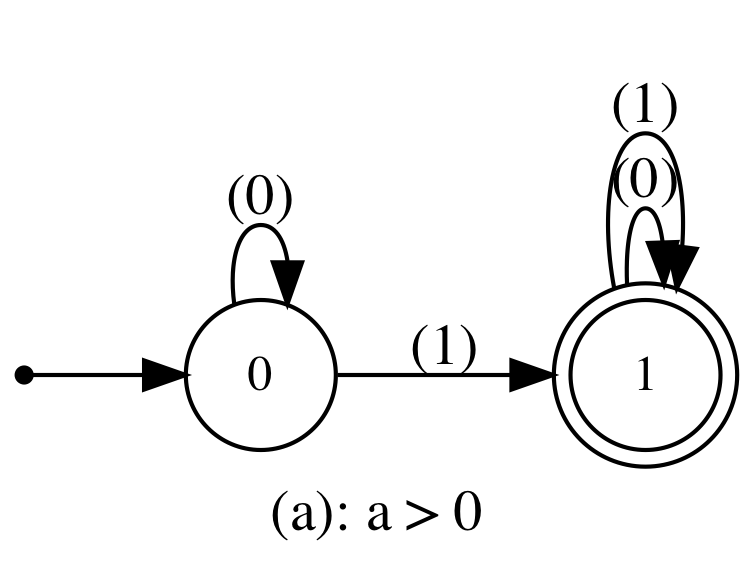
\includegraphics[height=0.45\textheight]{images/buchi_ex.jpg}
            \caption{B\"uchi automaton accepting all nonzero words}
        \end{figure}
\end{frame}


\begin{frame}{Creating an Automated Theorem Prover: Pecan}
    \frametitle{Creating an Automated Theorem Prover: Pecan}
    
\begin{table}[]
\begin{tabular}{|c|c|c|}
\hline
& \textbf{Walnut}  & \textbf{Pecan} \\ \hline
\multirow{3}{*}{\textbf{Inputs}}       & Predicates about & Predicates about \\

  & finite words    & infinite words \\\cline{2-3}
  & \multicolumn{2}{c|}{A first order statement of the predicates.} \\\hline

\textbf{Works using}                   & Finite automata  & B\"uchi automata   \\\hline
\textbf{Output} & \multicolumn{2}{c|}{An automaton for when the statement is correct. }\\\hline
\end{tabular}
\end{table}
    
\end{frame}

\section{Future Work}
\begin{frame}
  \frametitle{Future work}
  \begin{enumerate}
  \item Continue last semester's work on proving statements about \emph{every} Sturmian words using Pecan. For example prove or disprove that every Sturmian word contains grouped factors. 
  
  \item Prove properties about real numbers using Pecan since Pecan accepts infinite words.

  \end{enumerate}
  
\end{frame}


\end{document}